Die Ortsänderung ist die Fläche zwischen dem $v(t)$-Graphen und der $t$-Achse, unter der Achse negativ:
\begin{center}
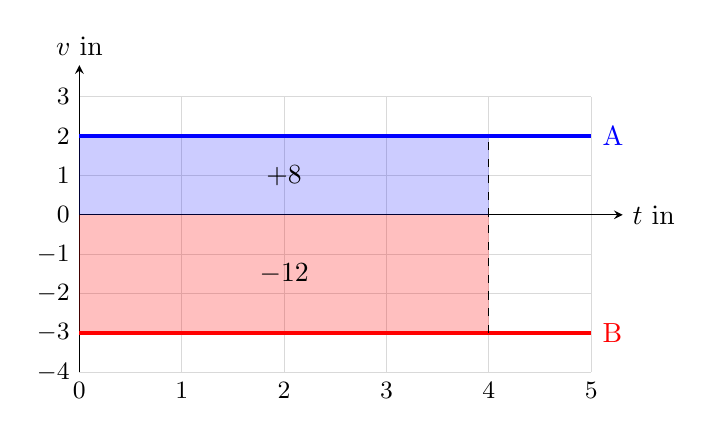
\begin{tikzpicture}[>=stealth, x=1.3cm, y=0.5cm]
 \draw[gray!30] (0,-4) grid[xstep=1, ystep=1] (5,3);
 \draw[->] (0,0) -- (5.308,0) node[right] {$t$ in \si{\second}};
 \draw[->] (0,-4) -- (0,3.8) node[above] {$v$ in \si{\meter\per\second}};
 \foreach \tk in {0,1,2,3,4,5} \node[below] at (\tk,-4) {\small $\tk$};
 \foreach \yk in {-4,-3,-2,-1,0,1,2,3} \node[left] at (0,\yk) {\small $\yk$};

 \fill[blue, opacity=0.2] (0,0) rectangle (4,2);
 \fill[red, opacity=0.25] (0,0) rectangle (4,-3);
 \draw[ultra thick, blue] (0,2) -- (5,2) node[right] {A};
 \draw[ultra thick, red] (0,-3) -- (5,-3) node[right] {B};
 \draw[dashed] (4,-3) -- (4,2);
 \node at (2,1) {$+8$};
 \node at (2,-1.5) {$-12$};
\end{tikzpicture}
\end{center}
\begin{abcliste}
\abc
\begin{align}
 s_\mathrm{A} &= \sAF = \vA\cdot\tE = \sA \approx \sAP{0}{1} \\
 s_\mathrm{B} &= \sBF = \left(\vB\right)\cdot\tE = \sB \approx \sBP{0}{2}
\end{align}
A ist \sAP{0}{1} in die positive Richtung gefahren, B \SI{12}{\meter} in die negative Richtung. $\result{\text{B ist weiter vom Start entfernt}}$. Das negative Vorzeichen gibt nur die Richtung an; die Entfernung ist der Betrag $|s_\mathrm{B}| = \SI{12}{\meter} > \SI{8}{\meter}$. Dass der Graph von B unter dem von A liegt, heisst nicht, dass B weniger weit gekommen ist, sondern dass B in die andere Richtung fährt.

\abc Die beiden fahren in entgegengesetzte Richtungen:
\begin{align}
 d_\mathrm{AB} &= \dABF = \sA-\left(\sB\right) = \dAB \approx \result{\dABP{0}{2}}
\end{align}
\end{abcliste}
